% This example is meant to be compiled with lualatex or xelatex
% The theme itself also supports pdflatex
\PassOptionsToPackage{unicode}{hyperref}
\documentclass[aspectratio=1610, 9pt]{beamer}

% Load packages you need here
\usepackage{polyglossia}
\setmainlanguage{english}
\setotherlanguages{german}

\usepackage{csquotes}

\usepackage{amsmath}
\usepackage{mathrsfs}
\usepackage{amssymb}
\usepackage{mathtools}
\usepackage{hyperref}
\usepackage{bookmark}
\usepackage{emoji}
\usepackage{tikz}
\usepackage[compat=1.1.0]{tikz-feynman}
\usepackage{appendixnumberbeamer}
\usepackage{color}
\usepackage[most]{tcolorbox}
\tcbset{colback=yellow!10!white, colframe=red!50!black, 
        highlight math style= {enhanced, %<-- needed for the ’remember’ options
            colframe=red,colback=red!10!white,boxsep=0pt}
        }
\usepackage{empheq}
\newcommand*\widefbox[1]{\fcolorbox{tugreen}{white}{\hspace{2em}#1\hspace{2em}}}

\usepackage[
  locale=UK,                   % UK Einstellungen
  separate-uncertainty=true,   % immer Unsicherheit mit \pm
  per-mode=symbol-or-fraction, % / in inline math, fraction in display math
]{siunitx}

\usepackage{graphicx, caption, subcaption}

% load the theme after all packages

\usetheme[
  showtotalframes, % show total number of frames in the footline
  % dark, % optional dark theme, uncomment to use
]{tudo}

% Put settings here, like
\unimathsetup{
  math-style=ISO,
  bold-style=ISO,
  nabla=upright,
  partial=upright,
  mathrm=sym,
}

\usepackage[
  % style=numeric,
  % style=authoryear-ibid,
  % style=verbose,
  doi=false,
  style=phys,
  % sorting=none,
  backend=biber,
  autolang=hyphen,
  articletitle=false,
  chaptertitle=false,
  biblabel=brackets,
  eprint=false,
  pageranges=false,
  doi=false,
  % useauthor=false,
]{biblatex}
% Quellendatenbank
\addbibresource{lit.bib}

\DeclareCiteCommand{\citecustom}
  {\usebibmacro{prenote}}
  {\usebibmacro{citeindex}%
   \printnames{author}%
   \setunit{\labelnamepunct}\newblock
   \printfield{title}%
   \setunit{\addcomma\space}%
   \printfield{eprint}%
   }
  {\multicitedelim}
  {\usebibmacro{postnote}}
  \DeclareMathOperator{\Tr}{Tr}

\title{BSM seminar talk: Axion models and EFT}
\author{Can Toraman \& Theodor Zies}
\date{04.07.2024}
\institute[Department of physics]{Supervision: Prof. Dr. Gudrun Hiller}
\titlegraphic{
\includegraphics[width=0.8\textwidth]{logos/Axion.jpeg}}

\captionsetup[figure]{labelformat=empty}
\captionsetup[table]{labelformat=empty}


\begin{document}

\begin{frame}
\titlepage
\end{frame}

\begin{frame}{Overview}
  \begin{columns}
    \column{\textwidth}
    \begin{itemize}
      \item Table of contents:
      \begin{itemize}
        \item [1.] Introduction
        \item [2.] Field theory axions
        \item [3.] String theory axions
        \item [4.] Axiverse from an EFT perspective
        \item [5.] Summary
      \end{itemize}
    \end{itemize}
    \begin{itemize}
      \item Talk based on \citecustom{paper}: "TASI Lectures on the Particle Physics and Astrophysics of Dark Matter"
    \end{itemize}
  \end{columns} 
\end{frame}

\begin{frame}[noframenumbering]
  \centering
  \Huge \textbf{\textcolor{tugreen}{Introduction}}
\end{frame}

\begin{frame}{Standard Model of Elementary Particles}
  \begin{columns}
    \centering
    \column{.5\textwidth}
    \begin{itemize}
      \item Standard Model of Particle Physics (SM) incomplete \\ (e.g. Dark Matter, Dark Energy, Neutrino masses)
      \item Search for New Physics (NP)
      \item Possible new particle candidate: Axions
      \item Axions could solve dark matter and strong CP problem
    \end{itemize}
    \column{.5\textwidth}
    \begin{figure}
    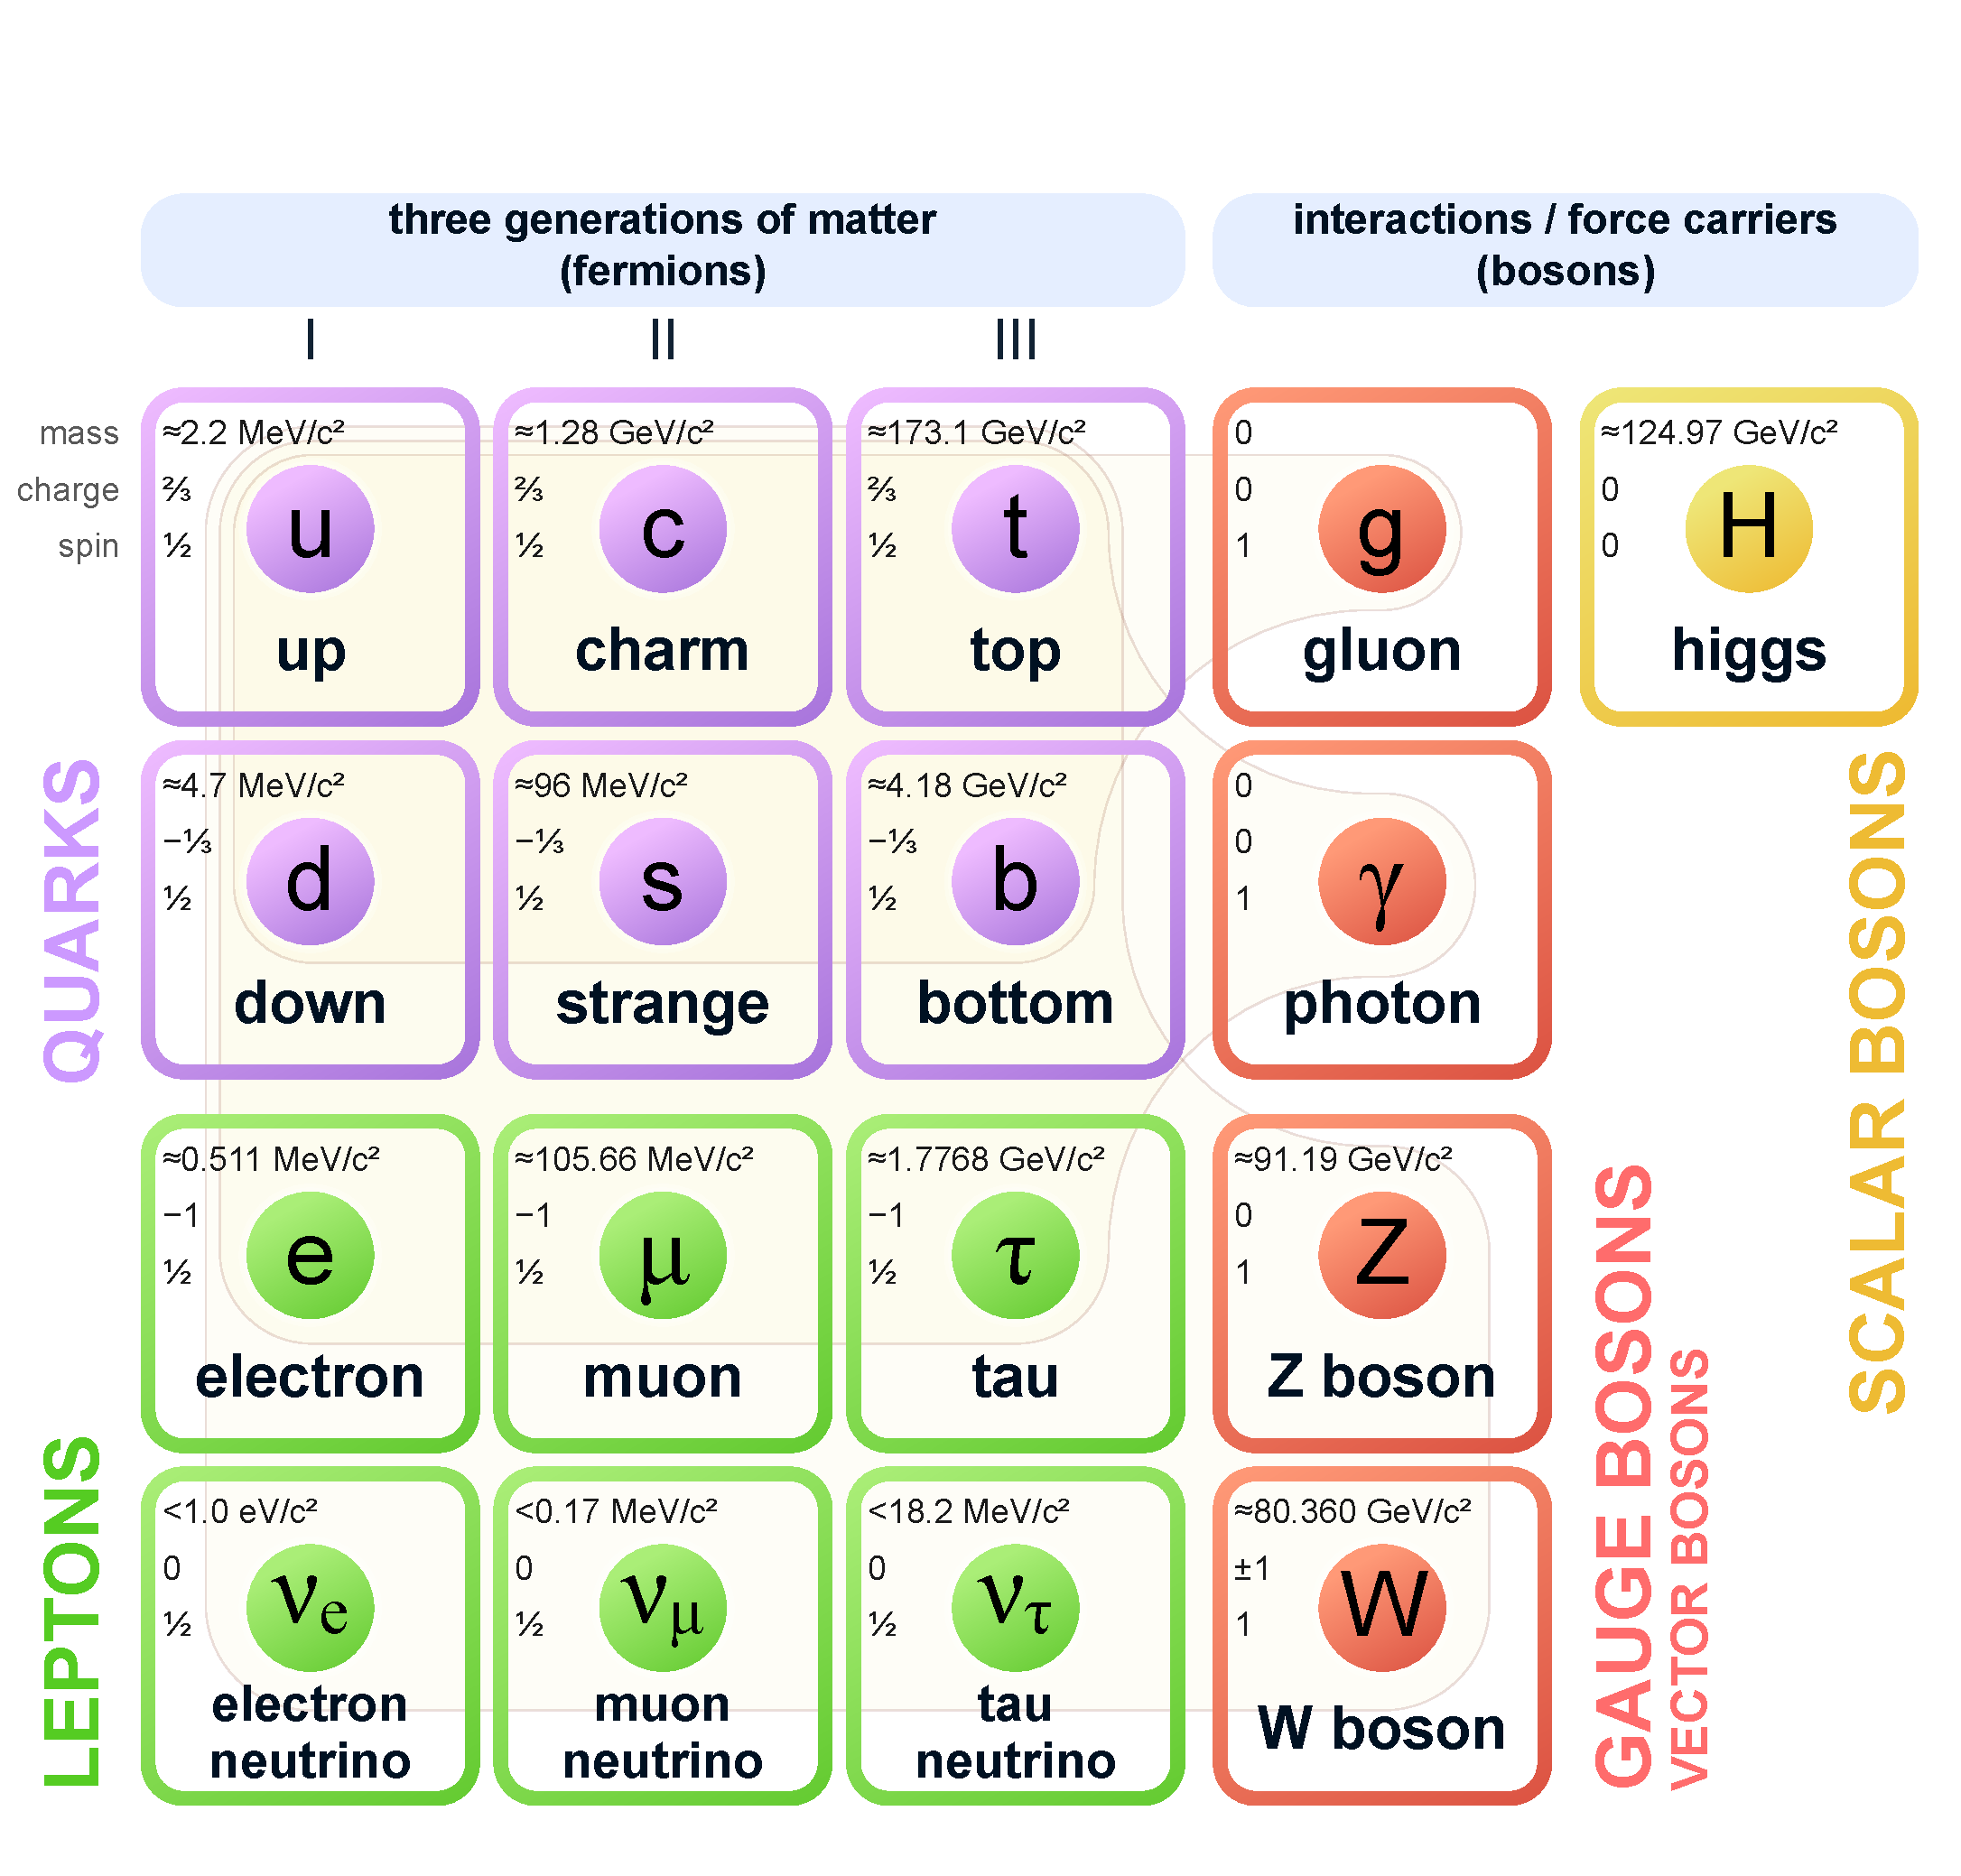
\includegraphics[height=6cm]{images/SM.pdf}
    \caption{\footnotesize \href{https://commons.wikimedia.org/wiki/File:Standard_Model_of_Elementary_Particles.svg}{{[commons.wikimedia.org]}}}
    \end{figure}
  \end{columns} 
\end{frame}

\begin{frame}{Why Axions?}
  \begin{columns}
    \column{.5\textwidth}
    \begin{itemize}
      \item QCD allows for CP violation in SM\\
      \begin{equation*}
      	\mathcal{L} = \frac{g_s^2}{32 \pi^2} \bar{\theta} G^a_{\mu \nu} \tilde{G}^{a \mu \nu}
      \end{equation*}
      \item Observe CP conservation in strong interaction $\rightarrow$ Strong CP problem
      \item Parameter $\bar{\theta}$ has to be fine tuned to be zero
      \item Physical meaning of $\bar{\theta}$: controls electric dipole moment of neutron
      \item Axions provide a dynamical explanation for lack of CP violation
      \item Dark matter is also explainable through axions
    \end{itemize}
    \column{.5\textwidth}
      \begin{figure}
      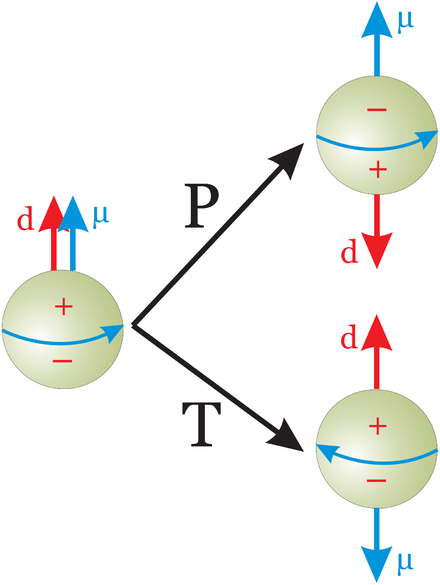
\includegraphics[height=6cm]{images/nEDM.png}
      \caption{\footnotesize \href{https://commons.wikimedia.org/wiki/File:NEDM_P26T_violation.png}{{[commons.wikimedia.org]}}}
      \end{figure}
  \end{columns} 
\end{frame}


\begin{frame}{Effective axion implementation}
  \begin{columns}
    \column{\textwidth}
    \begin{itemize}
      \item Introduce a massless, pseudo-scalar field $a(x)$ that has the dimension-five interaction with QCD:
    \end{itemize}
    \begin{equation*}
      \mathcal{L} \supset \frac{1}{2} \partial_\mu a \partial^\mu a - \frac{g_s^2}{32 \pi^2} \frac{a}{f_a} G^a_{\mu \nu} \tilde{G}^{a \mu \nu}
    \end{equation*}
    \begin{itemize}
      \item $f_a > 10^{9} \, \text{GeV}$ is the UV cut-off of the theory
      \item The QCD axion potential $V(a)$ is minimal if $\bar{\theta} = - \frac{a}{f_a} $
    \end{itemize}
    \begin{equation*}
      V(a) = -F_{\pi}^2 m_{\pi}^2 \sqrt{1 - 4 \frac{m_u m_d}{(m_u + m_d)^2} \sin \left( \frac{1}{2} \left( \bar{\theta} + \frac{a}{f_a} \right) \right)^2 }
    \end{equation*}
    \begin{itemize}
      \item CP violating term cancels
      \item Axions aquire a small mass:
    \end{itemize}
    \begin{equation*}
      m_a \approx \frac{F_{\pi} m_{\pi}}{f_a} \approx 6.0 \times 10^{-6} \left( \frac{10^{12} \, \text{GeV}}{f_a} \right) \text{eV}
    \end{equation*}
  \end{columns} 
\end{frame}

\begin{frame}{Axion models}
  \begin{columns}
    \column{\textwidth}
    \begin{itemize}
    \item Many different axion models exist
    \item Goal: Describe how effective axion arises from UV physics
    \end{itemize}
    \begin{enumerate}
      \item Field theory
      \item Extra dimensions, string theory
      \item Axiverse from an EFT perspective
    \end{enumerate}
  \end{columns} 
\end{frame}

\begin{frame}[noframenumbering]
  \centering
  \Huge \textbf{\textcolor{tugreen}{Field theory axions}}
\end{frame}

\begin{frame}{Field theory axion models}
  \begin{columns}
    \column{\textwidth}
    \begin{itemize}
      \item Axion emerging as pseudo-Goldstone boson of a $U(1)_{\text{PQ}}$ symmetry, known as the Peccei-Quinn (PQ) symmetry
      \item Axion is massless
      \item PQ symmetry is spontaneously broken below high scale $f_a$
      \item Introduce complex scalar field $\Phi$ with vacuum expectation value $v_a$:
    \end{itemize}
    \begin{equation*}
      \Phi(x) = \frac{r(x)+v_a}{\sqrt{2}}\exp \left(i\frac{a(x)}{v_a}\right) 
    \end{equation*}
    \begin{itemize}
    \item The PQ Langrangian allows spontaneous symmetry breaking:
    \end{itemize}
    \begin{align*}
      \mathcal{L}_{\Phi} &= \frac{1}{2} \partial_\mu \Phi \partial^\mu \Phi^\dagger - V(\Phi) \\
      & =  {| \partial_\mu \Phi |}^2 - \lambda \left( |\Phi|^2 - \frac{v_a^2}{2} \right)^2
    \end{align*}
  \end{columns} 
\end{frame}

\begin{frame}{Kim-Shifman-Vainshtein-Zakharov (KSVZ) model}
  \begin{columns}
    \column{\textwidth}
    \begin{itemize}
      \item Add $N$ identical vector-like fermions $Q_i$, $i=1,2,..,N$
      \item Charges (3, 1, 0) under $SU(3)_c × SU(2)_L × U(1)_Y$ symmetry
      \item Take $\Phi$ to be a SM singlet
      \item Write down the interaction terms between the $Q_i$ and $\Phi$:
    \end{itemize}
    \begin{equation*}
      \mathcal{L}_{\text{int}} = \sum_i \bar{Q}_i i \not{D} Q_i - \sum_i \left( y_i \bar{Q}_i Q_i \Phi + \text{h.c.} \right)
    \end{equation*}
    \begin{itemize}
      \item $y_i$ are Yukawa coupling constants
    \end{itemize}
  \end{columns} 
\end{frame}

\begin{frame}{Arriving at the EFT axion (1/2)}
  \begin{columns}
    \column{\textwidth}
    \begin{itemize}
      \item The full langrangian is invariant if the following symmetries hold:
    \end{itemize}
    \begin{align*}
      \Phi \rightarrow \Phi' &= e^{i \alpha} \Phi \quad U(1)_{\text{PQ}} \,\, \text{symmetry} \\
      Q_i \rightarrow Q_i' &= e^{\frac{i \alpha \gamma_5}{2}} \Phi \quad \text{Anomalous symmetry}
    \end{align*}
    \begin{itemize}
      \item At low energy scales $r(x) \ll v_a$:
    \end{itemize}
    \begin{equation*}
      \Phi(x) \rightarrow \frac{v_a}{\sqrt{2}}\exp \left( i\frac{a(x)}{v_a} \right) 
    \end{equation*}
    \begin{itemize}
      \item Substitute into $\mathcal{L}_{\text{int}}$ and define quark masses $m_i = \frac{y_i v_a}{\sqrt{2}}$:
    \end{itemize}
    \begin{equation*}
      \mathcal{L}_{\text{int}} = \sum_i \bar{Q}_i i \not{D} Q_i - \sum_i \left( m_i \bar{Q}_i Q_i \exp \left( i\frac{a(x)}{v_a} \right) + \text{h.c.} \right)
    \end{equation*}
  \end{columns} 
\end{frame}

\begin{frame}{Arriving at the EFT axion (2/2)}
  \begin{columns}
    \column{\textwidth}
    \begin{itemize}
      \item Apply the axial transformation to the quark fields (anomalous symmetry)
      \item Axion is removed from the interaction langrangian
      \item Following new term is induced:
    \end{itemize}
    \begin{equation*}
      \mathcal{L} \supset \frac{g_s^2}{32\pi^2} \frac{a}{v_a} N G^a_{\mu\nu} \tilde{G}^{a\mu\nu}
    \end{equation*}
    \begin{itemize}
      \item Exactly the dimension-five interaction with QCD if:
    \end{itemize}
    \begin{equation*}
      f_a = \frac{v_a}{N}
    \end{equation*}
    \begin{itemize}
      \item Integer $N$ known as \textit{domain wall number}
      \item Heavy fermion $Q$ is integrated out at the low scale
    \end{itemize}
  \end{columns} 
\end{frame}

\begin{frame}{Problems of the field theory axion}
  \begin{columns}
    \column{.5\textwidth}
    \begin{itemize}
      \item $N>1$ raises cosmological problems in UV completion of the theory
      \item Axion theories face "PQ quality problem"
      \item PQ symmetry needs to be a really good symmetry
      \item Problematic in picture of quantum gravity
      \item Quantum gravity not expected to conserve global symmetries \rightarrow black holes
    \end{itemize}
    \column{.5\textwidth}
    \begin{figure}
    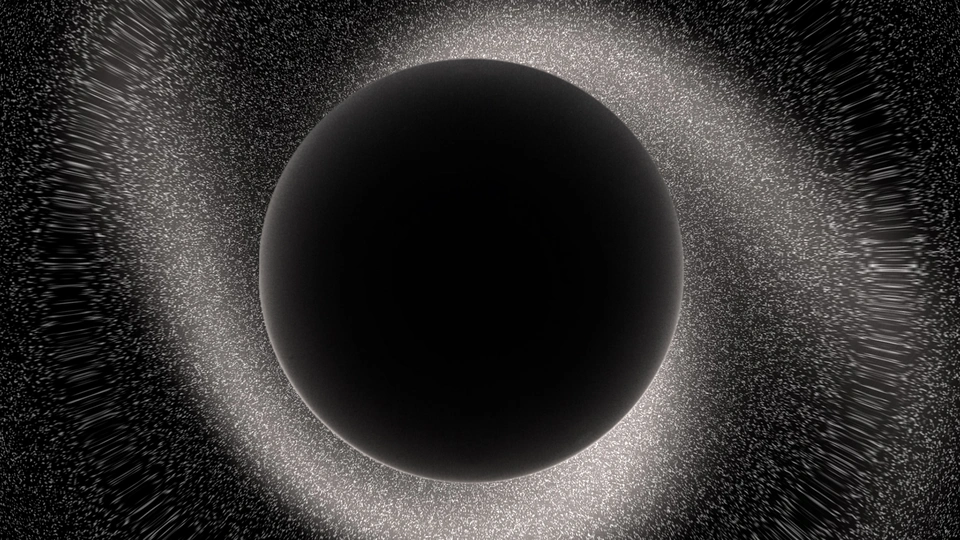
\includegraphics[height=4cm]{images/hole.png}
    \caption{\footnotesize \href{https://www.theatlantic.com/science/archive/2021/03/black-hole-cygnus-suprise/618049/}{{[theatlantic.com]}}}
    \end{figure}
  \end{columns}
\end{frame}

\begin{frame}{Breaking the PQ symmetry}
  \begin{columns}
    \column{\textwidth}
    \begin{itemize}
      \item Black holes should violate the global symmetry
      \item Break the symmetry at the planck scale $m_{\text{pl}}$:
    \end{itemize}
    \begin{equation*}
      \mathcal{L} \supset \lambda \frac{|\Phi|^{2n} \Phi^m}{m_{\text{pl}}^{2n+m-4}} + \text{h.c.}
    \end{equation*}
    \begin{itemize}
      \item $n$ and $m$ are integers, $\lambda$ is dimensionless coupling constant
      \item New relation with $\bar{\theta}$ arises:
    \end{itemize}
    \begin{equation*}
      \langle a \rangle + \bar{\theta} \sim \lambda \left( \frac{f_a}{m_{\text{pl}}} \right)^{2n+m} \left( \frac{m_{\text{pl}}}{\Lambda_{\text{QCD}}} \right)^4
    \end{equation*}
    \begin{itemize}
      \item $n$ and $m$ have to be very large or $\lambda$ really small
      \item New fine tuning problem, because otherwise $\bar{\theta}$ is not close to zero
    \end{itemize}
  \end{columns} 
\end{frame}

\begin{frame}[noframenumbering]
  \centering
  \Huge \textbf{\textcolor{tugreen}{String theory axions}}
\end{frame}

\begin{frame}
	\frametitle{String Theory}
	\begin{minipage}{0.55\textwidth}
		\begin{itemize}
			\item Why do we need String Theory?\\
			$\rightarrow$ Quantum Gravity (QG) violates $PQ$-Symmetry
			\item String Theory (ST) is a theory of QG
			\item Some particles proposed in ST are good axion candidates\\
			\item Requirements
			\begin{itemize}
				\item[(1)] Scalar particle
				\item[(2)] High PQ Quality and spontaneous breaking
				\item[(3)] QCD Contribution (Strong CP violation)\\
				\begin{equation*}
					\mathcal{L} \supset \frac{g_s^2}{32 \pi^2} \frac{a}{f_a} G^a_{\mu \nu} \tilde{G}^{a \mu \nu}
				\end{equation*}
				\item[(4)] Sufficiently low mass/coupling (Fit experimental bounds)
				%				\item[(5)]
			\end{itemize}			
			
		\end{itemize}
	\end{minipage}
	\hfill
	\begin{minipage}{0.4\textwidth}
		\begin{figure}
			\centering
			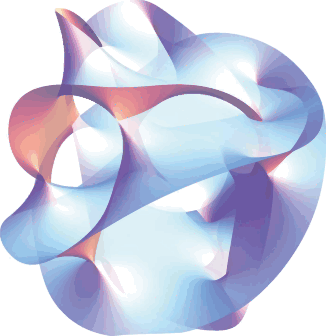
\includegraphics[width=4.5cm]{images/string.pdf}
			\caption{\href{https://en.wikipedia.org/wiki/File:Calabi_yau_formatted.svg}{[commons.wikimedia]}}
		\end{figure}
	\end{minipage}
%	\footnotetext[1]{\protect\footnotesize \fullcite{}}
\end{frame}

\begin{frame}
	\frametitle{String Theory - Overview}
	\begin{minipage}{0.7\textwidth}
		\begin{itemize}
			\item Idea: Particles are points $\rightarrow$ Stings in higher dimension (open or closed)\\
			$\rightarrow$ Different vibrational modes represent different particles
			\item Multiple different theories under the term ST
			\item All expand the dimensionality to 10, 11 or 26\\
			$\rightarrow$ Compactification used to create a 4D representation of these strings
			\item Extra dimensions are infinite
			\item Different topology leads to different shapes $\rightarrow$ different physical consequences (generation, gauge groups etc.)
			\item Compactification $\rightarrow$ curls the infinite dimensions up into a finite geometrical shape (e.g. a circle) %by e.g. integrating over the finite extra dimensions
			
		\end{itemize}
	\end{minipage}
	\hfill
	\begin{minipage}{0.25\textwidth}
			\begin{figure}
					\centering
					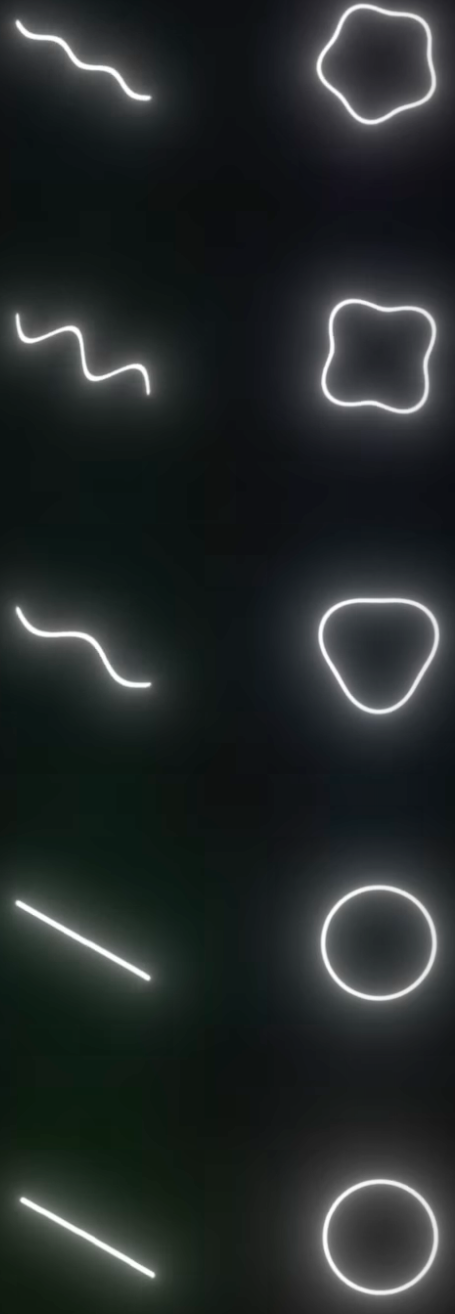
\includegraphics[width=2.25cm]{images/modes.png}
          \caption{\href{https://www.youtube.com/watch?v=n7cOlBxtKSo}{[youtube.com/ScienceClic English]}}
				\end{figure}
		\end{minipage}
\end{frame}

\begin{frame}
	\frametitle{Types of String Theories}
		\begin{itemize}
			\item Bosonic String Theory\\
			$\rightarrow$ Most simple case (26 Dimensions) 
			\item Superstring Theory (10 Dimensions, Supersymmetry $\rightarrow$ Each boson has a fermion partner)\\
			\begin{itemize}
				\item[\ ]{\color{tugreen!60!black}Type I:}\ \ \ \ Both closed and open strings
				\item[\ ]{\color{tugreen!60!black}Type IIA:} Only closed and non-chiral (no distinguishing between LH or RH particles)
				\item[\ ]{\color{tugreen!60!black}Type IIB:} Also only closed but chiral $\rightarrow$ Good axion like particles
				\item[\ ]{\color{tugreen!60!black}And others}
			\end{itemize}
			\item M-Theory (11 Dimensions)
			$\rightarrow$ Attempt to unify all Superstring Theories
		\end{itemize}
\end{frame}


\begin{frame}
	\frametitle{5D Example}
	
	\begin{itemize}
		\item Coordinates: $(x_0, x_1, x_2, x_3, y)$, with y compactified on a circle (Radius $R$) 
		\item The fifth dimension y is modded out under a symmetry $Z_2$ (objects transformed in this dimensions remain even)
		\item We introduce a $U(1)$ gauge field $B_M$ with $M = 0,1,2,3,5$, which transform under $Z_2$ like:
		\begin{equation*}
			B_{\mu}(-y) = -B_{\mu}(y)\hspace{1 cm}\text{and}\hspace{1cm}  B_5(-y) = B_5(y)
		\end{equation*}	
		\item One additional gauge field $F_M$ is introduced (Field strength tensor $F_{MN}$)
		\item This leads to the following Lagrangian terms
		\begin{equation*}
			\mathcal{L}_{5D} \supset \int d^4x \int_0^{2\pi R} dy \left( \frac{1}{4 g_5^2} B_{MN} B^{MN} + \kappa \epsilon^{MNPQR} B_M \Tr(F_{NP} F_{QR}) \right)
		\end{equation*}
		$g_5$, $\kappa$ coupling constants, $\epsilon^{MNPQR}$ totally antisymmetric tensor
	\end{itemize}
\end{frame}

\begin{frame}
	\frametitle{5D Example}
		\begin{itemize}
			\item Introduction of the axion as $B_M$ zero-modes (Massless compactification of the Field)\\
			$\rightarrow$ Axion field is defined as: 
			\begin{equation*}
				{\Large e^{2\pi R i a} \equiv e^{i\int_{0}^{2\pi R}B_5(x_\mu, y)dy}}
			\end{equation*}
			We assume for simplicity $\int_{0}^{2\pi R}B_5(x_\mu, y)dy = 2\pi RB_5(x_\mu, y)$
			\item Plugging it into:
			\begin{equation*}
				\mathcal{L}_{4D} \supset \int d^4x \int_0^{2\pi R} dy \left( \frac{1}{4 g_5^2} \underbrace{B_{MN} B^{MN}}_{\rightarrow\ B_{\mu\nu}B^{\mu\nu} + 2(\partial_\mu a)^2} + \kappa \underbrace{\epsilon^{MNPQR} B_M \Tr(F_{NP} F_{QR})}_{\rightarrow aF_{\mu\nu}^a \tilde{F}^{a\mu\nu}} \right)
			\end{equation*}
			\item After integrating:
			\begin{equation*}
				\mathcal{L}_{4D} \supset \int d^4x \left( \frac{2\pi R}{2g_5^2} (\partial_\mu a)^2 + (2\pi R \kappa) a F_{\mu\nu}^a \tilde{F}^{a\mu\nu} \right)
			\end{equation*}
		\end{itemize}
\end{frame}

\begin{frame}
	\frametitle{5D Example}
	\begin{itemize}
		\item To form the CPV term we chose:
		\begin{equation*}
			f_a = \frac{1}{32 \sqrt{3} \pi^{5/2} \kappa} \frac{1}{g_5 \sqrt{R}} = \frac{1}{64 \pi^3 \kappa g_4} \frac{1}{R}
		\end{equation*}
		\item Finally we obtain:
		\begin{equation*}
			\mathcal{L}_{4D} \supset \int d^4x \left( \frac{1}{2} (\partial_\mu a)^2 + \frac{g_f^2}{32 \pi^2} \frac{a}{f_a} F_{\mu\nu}^a \tilde{F}^{a\mu\nu} \right)
		\end{equation*}
		$\rightarrow$ PQ-Symmetry broken for low energy solutions
    \item Higher dimension string theories give rise to a multitude of axions or axion like particles (depending on topology)
	\end{itemize}
\end{frame}

\begin{frame}[noframenumbering]
  \centering
  \Huge \textbf{\textcolor{tugreen}{Axiverse from an EFT perspective}}
\end{frame}

\begin{frame}{The Axiverse}
  \begin{columns}
    \column{\textwidth}
    \begin{itemize}
      \item String theory compactifications tend to predict large numbers of axion like particles (ALP)
      \item Axions have QCD induced masses and explicit masses
      \item Explicit axion masses are set by exponential factors
      \item Expect roughly logarithmic distribution of ALP masses over a large mass range
      \item Potentially from well below e.g. $10^{-22}$ eV to values $10^{-10}$ eV or higher
    \end{itemize}
    \vspace{1cm}
    \centering
    \rightarrow Universe full of very light axions, the "axiverse"
  \end{columns} 
\end{frame}

\begin{frame}{From an EFT perpective}
  \begin{columns}
    \column{\textwidth}
    \begin{itemize}
      \item Implement $N$ axions with the following set of dimension-five interactions with the SM:
    \end{itemize}
    \begin{equation*}
      \mathcal{L} \supset \sum_{i=1}^{N} \left[ \frac{g_s^2}{32\pi^2} \frac{c_s^i a_i}{f_a} G_{\mu\nu}^a \tilde{G}^{a\mu\nu} 
    + \frac{g_2^2}{32\pi^2} \frac{c_2^i a_i}{f_a} W_{\mu\nu}^a \tilde{W}^{a\mu\nu} 
    + \frac{g_1^2}{32\pi^2} \frac{c_1^i a_i}{f_a} B_{\mu\nu} \tilde{B}^{\mu\nu} 
    + \sum_f C_{aff} \frac{\partial_\mu a_i}{2f_a} \bar{f} \gamma^\mu \gamma_5 f 
    - \frac{1}{2} (m_i^0)^2 a_i^2 \right]
    \end{equation*}
    \begin{itemize}
      \item Assume that bare masses $m_i^0$ are small relative to the ones induced by QCD: $ \frac{\Lambda^2}{f_a} \ll m_i^0$
      \item Diagonalizing the mass matrix yields almost pure mass eigenstate:
    \end{itemize}
    \begin{equation*}
      a_{\text{QCD}} = \frac{\sum_{i} c_{s}^{i} a_{i}}{\sum_{i} (c_{s}^{i})^2}
    \end{equation*}
    \begin{itemize}
      \item QCD axion with mass $ m_{\text{QCD}} ≈ \Lambda_{\text{QCD}}^2 / f_a $
      \item Remaining N-1 ALPS are verly light and do not couple to QCD
      \item Below the electroweak scale the axion and ALPs acquire couplings to electromagnetism
    \end{itemize}
  \end{columns} 
\end{frame}

\begin{frame}[noframenumbering]
  \centering
  \Huge \textbf{\textcolor{tugreen}{Summary}}
\end{frame}

\begin{frame}{Summary}
  \begin{columns}
    \column{\textwidth}
    \begin{itemize}
      \item Axions can provide promising solution for the strong CP problem and dark matter
      \item NP models try to motivate axion existence at high energy scale
      \begin{itemize}
				\item[(1)] Field theory axion problematic in respect to QG
				\item[(2)] String theory naturally produces axions while encompassing QG
				\item[(3)] The string theory axiverse can be implemented as an EFT
      \end{itemize}
      \item Due to low mass and small coupling with SM, no evidence for axions has been oberved yet
    \end{itemize}
    \vspace{1cm}
    \centering
    \textbf{\Huge{\textcolor{tugreen}{Thank you for your attention!}}}
  \end{columns} 
\end{frame}

\end{document}